\documentclass[journal,12pt,twocolumn]{IEEEtran}
%
\usepackage{setspace}
\usepackage{gensymb}
\usepackage{xcolor}
\usepackage{caption}
%\usepackage{subcaption}
%\doublespacing
\singlespacing

%\usepackage{graphicx}
%\usepackage{amssymb}
%\usepackage{relsize}
\usepackage[cmex10]{amsmath}
\usepackage{mathtools}
%\usepackage{amsthm}
%\interdisplaylinepenalty=2500
%\savesymbol{iint}
%\usepackage{txfonts}
%\restoresymbol{TXF}{iint}
%\usepackage{wasysym}
\usepackage{hyperref}
\usepackage{amsthm}
\usepackage{mathrsfs}
\usepackage{txfonts}
\usepackage{stfloats}
\usepackage{cite}
\usepackage{cases}
\usepackage{subfig}
%\usepackage{xtab}
\usepackage{longtable}
\usepackage{multirow}
%\usepackage{algorithm}
%\usepackage{algpseudocode}
%\usepackage{enumerate}
\usepackage{enumitem}
\usepackage{mathtools}
%\usepackage{iithtlc}
%\usepackage[framemethod=tikz]{mdframed}
\usepackage{listings}
\let\vec\mathbf
\usepackage{circuitikz}

%\usepackage{stmaryrd}


%\usepackage{wasysym}
%\newcounter{MYtempeqncnt}
\DeclareMathOperator*{\Res}{Res}
%\renewcommand{\baselinestretch}{2}
\renewcommand\thesection{\arabic{section}}
\renewcommand\thesubsection{\thesection.\arabic{subsection}}
\renewcommand\thesubsubsection{\thesubsection.\arabic{subsubsection}}

\renewcommand\thesectiondis{\arabic{section}}
\renewcommand\thesubsectiondis{\thesectiondis.\arabic{subsection}}
\renewcommand\thesubsubsectiondis{\thesubsectiondis.\arabic{subsubsection}}

%\renewcommand{\labelenumi}{\textbf{\theenumi}}
%\renewcommand{\theenumi}{P.\arabic{enumi}}

% correct bad hyphenation here
\hyphenation{op-tical net-works semi-conduc-tor}

\lstset{
language=Python,
frame=single, 
breaklines=true,
columns=fullflexible
}



\begin{document}
%

\theoremstyle{definition}
\newtheorem{theorem}{Theorem}[section]
\newtheorem{problem}{Problem}
\newtheorem{proposition}{Proposition}[section]
\newtheorem{lemma}{Lemma}[section]
\newtheorem{corollary}[theorem]{Corollary}
\newtheorem{example}{Example}[section]
\newtheorem{definition}{Definition}[section]
%\newtheorem{algorithm}{Algorithm}[section]
%\newtheorem{cor}{Corollary}
\newcommand{\BEQA}{\begin{eqnarray}}
\newcommand{\EEQA}{\end{eqnarray}}
\newcommand{\define}{\stackrel{\triangle}{=}}
\newcommand{\myvec}[1]{\ensuremath{\begin{pmatrix}#1\end{pmatrix}}}
\newcommand{\mydet}[1]{\ensuremath{\begin{vmatrix}#1\end{vmatrix}}}

\bibliographystyle{IEEEtran}
%\bibliographystyle{ieeetr}

\providecommand{\nCr}[2]{\,^{#1}C_{#2}} % nCr
\providecommand{\nPr}[2]{\,^{#1}P_{#2}} % nPr
\providecommand{\mbf}{\mathbf}
\providecommand{\pr}[1]{\ensuremath{\Pr\left(#1\right)}}
\providecommand{\qfunc}[1]{\ensuremath{Q\left(#1\right)}}
\providecommand{\sbrak}[1]{\ensuremath{{}\left[#1\right]}}
\providecommand{\lsbrak}[1]{\ensuremath{{}\left[#1\right.}}
\providecommand{\rsbrak}[1]{\ensuremath{{}\left.#1\right]}}
\providecommand{\brak}[1]{\ensuremath{\left(#1\right)}}
\providecommand{\lbrak}[1]{\ensuremath{\left(#1\right.}}
\providecommand{\rbrak}[1]{\ensuremath{\left.#1\right)}}
\providecommand{\cbrak}[1]{\ensuremath{\left\{#1\right\}}}
\providecommand{\lcbrak}[1]{\ensuremath{\left\{#1\right.}}
\providecommand{\rcbrak}[1]{\ensuremath{\left.#1\right\}}}
\providecommand{\rect}[1]{\text{rect}\ensuremath{\left(#1\right)}}
\providecommand{\sinc}[1]{\text{sinc}\ensuremath{\left(#1\right)}}
\theoremstyle{remark}
\newtheorem{rem}{Remark}
\newcommand{\sgn}{\mathop{\mathrm{sgn}}}
\providecommand{\abs}[1]{\left\vert#1\right\vert}
\providecommand{\res}[1]{\Res\displaylimits_{#1}} 
\providecommand{\norm}[1]{\lVert#1\rVert}
\providecommand{\mtx}[1]{\mathbf{#1}}
\providecommand{\mean}[1]{E\left[ #1 \right]}
\providecommand{\fourier}{\overset{\mathcal{F}}{ \rightleftharpoons}}
\providecommand{\ztrans}{\overset{\mathcal{Z}}{ \rightleftharpoons}}

%\providecommand{\hilbert}{\overset{\mathcal{H}}{ \rightleftharpoons}}
%\providecommand{\system}{\overset{\mathcal{H}}{ \longleftrightarrow}}
\providecommand{\system}[1]{\overset{\mathcal{#1}}{ \longleftrightarrow}}
	%\newcommand{\solution}[2]{\textbf{Solution:}{#1}}
\newcommand{\solution}{\noindent \textbf{Solution: }}
\providecommand{\dec}[2]{\ensuremath{\overset{#1}{\underset{#2}{\gtrless}}}}
\numberwithin{equation}{section}
%\numberwithin{equation}{subsection}
%\numberwithin{problem}{subsection}
%\numberwithin{definition}{subsection}
\makeatletter
\@addtoreset{figure}{problem}
\makeatother

\let\StandardTheFigure\thefigure
%\renewcommand{\thefigure}{\theproblem.\arabic{figure}}
\renewcommand{\thefigure}{\theproblem}


%\numberwithin{figure}{subsection}

\def\putbox#1#2#3{\makebox[0in][l]{\makebox[#1][l]{}\raisebox{\baselineskip}[0in][0in]{\raisebox{#2}[0in][0in]{#3}}}}
     \def\rightbox#1{\makebox[0in][r]{#1}}
     \def\centbox#1{\makebox[0in]{#1}}
     \def\topbox#1{\raisebox{-\baselineskip}[0in][0in]{#1}}
     \def\midbox#1{\raisebox{-0.5\baselineskip}[0in][0in]{#1}}

\vspace{3cm}

\title{ 
%\logo{
%}
Fourier Series
%	\logo{Octave for Math Computing }
}
%\title{
%	\logo{Matrix Analysis through Octave}{\begin{center}\includegraphics[scale=.24]{tlc}\end{center}}{}{HAMDSP}
%}


% paper title
% can use linebreaks \\ within to get better formatting as desired
%\title{Matrix Analysis through Octave}
%
%
% author names and IEEE memberships
% note positions of commas and nonbreaking spaces ( ~ ) LaTeX will not break
% a structure at a ~ so this keeps an author's name from being broken across
% two lines.
% use \thanks{} to gain access to the first footnote area
% a separate \thanks must be used for each paragraph as LaTeX2e's \thanks
% was not built to handle multiple paragraphs
%

\author{ VIBHAVASU - EP20BTECH11015 $^{}$}

% make the title area
\maketitle

%\newpage

\tableofcontents

%\renewcommand{\thefigure}{\thesection.\theenumi}
%\renewcommand{\thetable}{\thesection.\theenumi}

\renewcommand{\thefigure}{\theenumi}
\renewcommand{\thetable}{\theenumi}

%\renewcommand{\theequation}{\thesection}


\bigskip

\begin{abstract}
This manual provides a simple introduction to Fourier Series
\end{abstract}
\section{Periodic Function}
Let 
\begin{align}
	x(t) &= A_0\abs{\sin\brak{2\pi f_0 t}}
	\label{eq:10-orig-diff-def}
\end{align}
\begin{enumerate}[label=\thesection.\arabic*
,ref=\thesection.\theenumi]
\item Plot $x(t)$.\\
\solution
\begin{lstlisting}
https://github.com/DarkWake9/EE3900/blob/main/charger/codes/e1.1.py
\end{lstlisting}
\begin{figure}[!ht]
	\begin{center}
		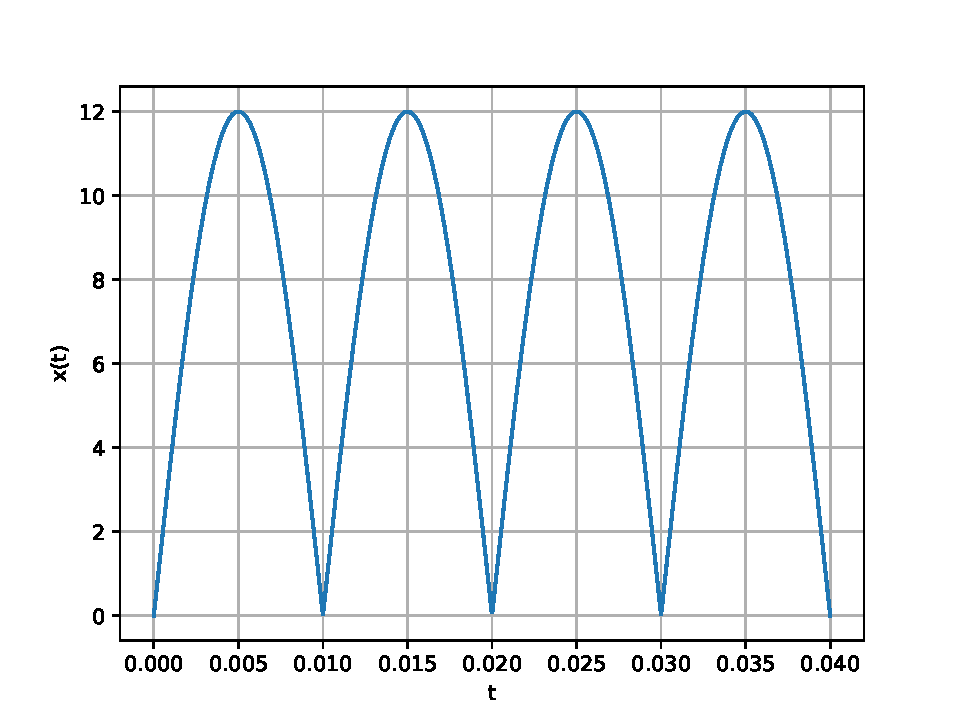
\includegraphics[width=\columnwidth]{./figs/e1.1.pdf}
	\end{center}
	\captionof{figure}{}
	\label{fig:xt}	
\end{figure}
\item Show that $x(t)$ is periodic and find its period.
\solution From Fig. \eqref{fig:xt}, we see that $x(t)$ is periodic. Further,
\begin{align}
	x\brak{t+\frac{1}{2f_0}} = A_0\abs{\sin\brak{2\pi f_0\brak{t + \frac{1}{2f_0}}}} \\
	= A_0\abs{\sin\brak{2\pi f_0t + \pi}} \\
	= A_0\abs{\sin\brak{2\pi f_0t}}
\end{align}
$\therefore$ \text{period of }$x(t)$ is $\dfrac{1}{2f_0}$.

\end{enumerate}
\section{Fourier Series}
Consider $A_0 =12$ and $f_0 = 50$ for all numerical calculations.
\begin{enumerate}[label=\thesection.\arabic*,ref=\thesection.\theenumi]
\item If
%\cite{proakis_dsp}
\begin{align}
	x(t) = \sum_{k = -\infty}^{\infty}c_ke^{\j2\pi kf_0 t}
\label{eq:one-Z-complex}
\end{align}
show that 
\begin{align}
	c_k = f_0\int_{-\frac{1}{2f_0}}^{\frac{1}{2f_0}}x(t)e^{-\j2\pi kf_0 t}\, dt
\label{eq:one-Z}
\end{align}
\solution\\
Multiplying both sides by $e^{-\j2\pi kf_0 t}$ Integrating w.r.t t from $-\frac{1}{2f_0}$ to ${\frac{1}{2f_0}}$:
\begin{align}
	\int_{-\frac{1}{2f_0}}^{\frac{1}{2f_0}}x(t)e^{-\j2\pi kf_0 t} dt\\
	 = \int_{-\frac{1}{2f_0}}^{\frac{1}{2f_0}} \brak{\sum_{n = -\infty}^{\infty}c_ne^{\j2\pi nf_0 t}}e^{-\j2\pi kf_0 t} dt\\
	 = \sum_{n = -\infty}^{\infty}c_n\int_{-\frac{1}{2f_0}}^{\frac{1}{2f_0}} e^{\j2\pi (n-k)f_0 t} dt\\
	 =\sum_{n = -\infty}^{\infty}c_n \frac{\delta(n-k)}{f_0}
	 =\frac{c_k}{f_0}\\
	\therefore c_k = f_0\int_{-\frac{1}{2f_0}}^{\frac{1}{2f_0}}x(t)e^{-\j2\pi kf_0 t}\, dt
\end{align}


\item Find $c_k$ for 
	\eqref{eq:10-orig-diff-def}\\
\solution\\
\begin{align}
	c_k &= \int_{-\frac{1}{2f_0}}^{\frac{1}{2f_0}} A_0 \abs{\sin(2\pi f_0 t)}e^{-\j2\pi kf_0 t} dt\\
	&= f_0\int_{-\frac{1}{2f_0}}^{\frac{1}{2f_0}}A_0\abs{\sin\brak{2\pi f_0t}}
	\cos\brak{2\pi nf_0t}\, dt \nonumber \\
	&+ \j f_0\int_{-\frac{1}{2f_0}}^{\frac{1}{2f_0}}A_0
	\abs{\sin\brak{2\pi f_0t}}\sin\brak{2\pi nf_0t}\, dt \\
	&= 2f_0\int_{0}^{\frac{1}{2f_0}}A_0\sin\brak{2\pi f_0t}\cos\brak{2\pi nf_0t}\, dt \\
	&= f_0A_0\int_{0}^{\frac{1}{2f_0}}\brak{\sin\brak{2\pi\brak{n+1}f_0t}}\, dt \nonumber \\ 
	&- f_0A_0\int_{0}^{\frac{1}{2f_0}}\brak{\sin\brak{2\pi\brak{n-1}f_0t}}\, dt \\ 
	&= A_0\frac{1+\brak{-1}^n}{2\pi}\brak{\frac{1}{n+1} - \frac{1}{n-1}} \\
	&= 
	\begin{cases}
		\frac{2A_0}{\pi\brak{1-n^2}} & n\ \text{even} \\
		0 & n\ \text{odd}
	\end{cases}
	\label{eq:ck-xt}
\end{align}
	
\item Verify 
	\eqref{eq:10-orig-diff-def}
	using python.
\begin{lstlisting}
https://github.com/DarkWake9/EE3900/blob/main/charger/codes/e2.3.py
\end{lstlisting}
\begin{figure}[!ht]
	\begin{center}
		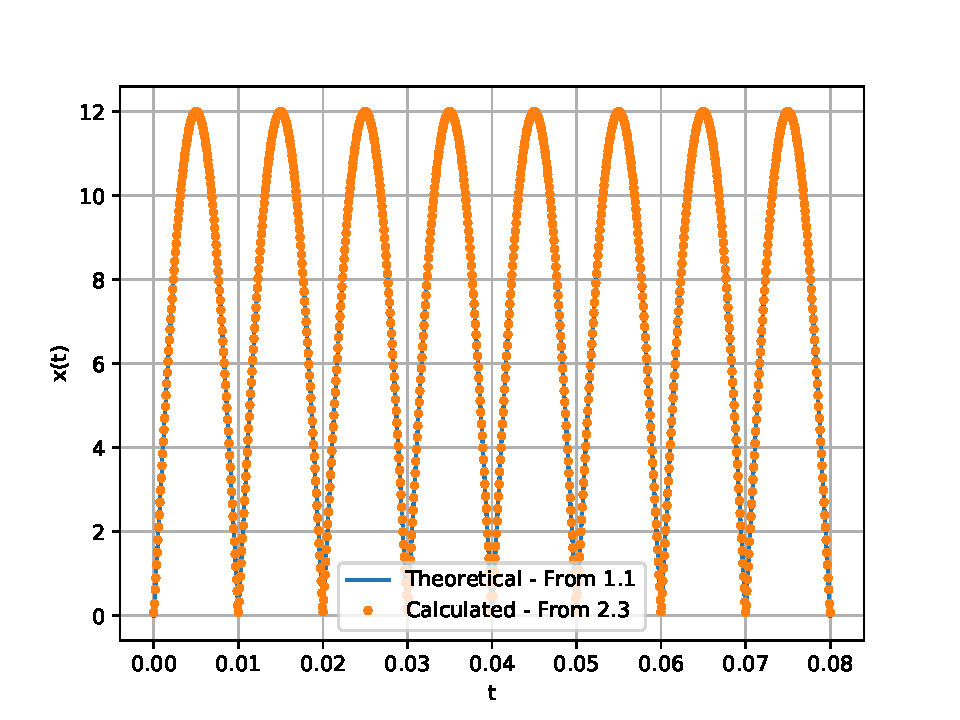
\includegraphics[width=\columnwidth]{./figs/e2.3.pdf}
	\end{center}
	\captionof{figure}{}
	\label{fig:}	
\end{figure}	

\item Show that 
\begin{align}
	x(t) = \sum_{k = 0}^{\infty}\brak{a_k\cos{\j2\pi kf_0 t}+b_k\sin{\j2\pi kf_0 t}}
\label{eq:one-Z-real}
\end{align}
and obtain the formulae for $a_k$ and $b_k$.\\
\solution\\
\begin{align}
	&x(t) = \sum_{k = -\infty}^{\infty}c_ke^{\j2\pi kf_0 t} \\
	&= c_0 + \sum_{k = 1}^{\infty}c_ke^{\j2\pi kf_0t} + c_{-k}e^{-\j2\pi kf_0t} \\
	&= c_0 + \sum_{k = 1}^{\infty}\brak{c_k + c_{-k}}\cos\brak{2\pi kf_0t}  \nonumber \\
	&+ \sum_{k = 0}^{\infty}\brak{c_k - c_{-k}}\sin\brak{2\pi kf_0t}
\end{align}

\begin{align}
	\implies
	a_k &= 
	\begin{cases}
		c_0 & k = 0 \\
		c_k + c_{-k} & k > 0
	\end{cases} \label{eq:ak} \\
	b_k &= c_k - c_{-k}
	\label{eq:bk}
\end{align}
\item Find $a_k$ and $b_k$ for 
\eqref{eq:10-orig-diff-def}\\
\solution\\
From \eqref{eq:10-orig-diff-def}:
\begin{align}
	x(-t) = x(t)\\
	\implies \sum_{k = -\infty}^{\infty}c_{-k}e^{\j2\pi kf_0t}
	= \sum_{k = -\infty}^{\infty}c_ke^{\j2\pi kf_0 t}\\
	\implies c_k = c_{-k}\\
	a_k = \begin{cases}
		\frac{2A_0}{\pi\brak{1-n^2}} \quad n\ = 0\\
		\frac{4A_0}{\pi\brak{1-n^2}} \quad n\ \text{ is even}\\
		0 \quad \text{otherwise}
	\end{cases}\\
	b_k = 0
\end{align}
\item Verify 
\eqref{eq:one-Z-real}
using python.
\begin{lstlisting}
https://github.com/DarkWake9/EE3900/blob/main/charger/codes/e2.6.py
\end{lstlisting}
\begin{figure}[!ht]
	\begin{center}
		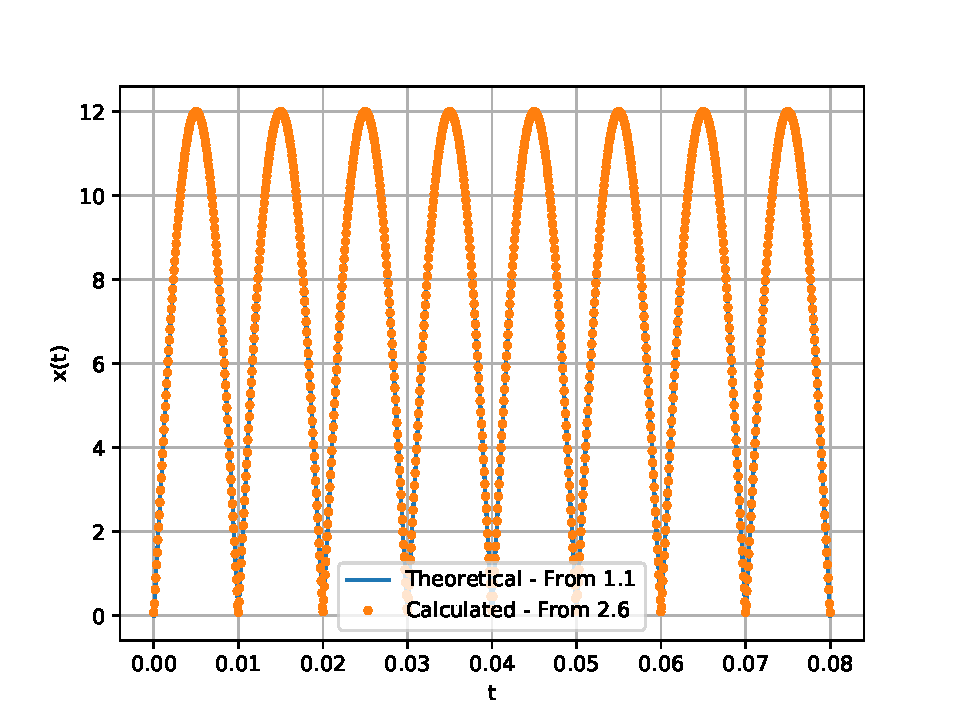
\includegraphics[width=\columnwidth]{./figs/e2.6.pdf}
	\end{center}
	\captionof{figure}{Fourier Expansion of x(t)}
	\label{fig:ft}	
\end{figure}
\end{enumerate}
\section{Fourier Transform}

 

\begin{enumerate}[label=\thesection.\arabic*
,ref=\thesection.\theenumi]
\item 
	\begin{align}
		\delta(t)&=0, \quad t\neq0
\\
		\int_{-\infty}^{\infty}\delta(t) \, dt&= 1
	\end{align}
 \item The Fourier Transform of $g(t)$ is
 \begin{align}
 G(f)=\int_{-\infty}^{\infty}g(t)e^{-j2\pi ft}\,dt
 \end{align}
 \item Show that 
 \begin{align}
	 g(t-t_0)&\system{F}G(f)e^{-j2\pi ft_0}
 \end{align}
\solution\\
Put $t-t_0 = t'$,
\begin{align}
	g(t-t_0) = g(t')\system{F}\int_{-\infty}^{\infty} g(t')e^{-\j2\pi ft}\,dt \\
	\int_{-\infty}^{\infty}	g(u)e^{-\j2\pi f(t' + t_0)}\,dt' \\
	=G(f)e^{-j2\pi ft_0}
\end{align}
 \item Show that 
 \begin{align}
	 G(t)&\system{F}g(-f)
 \end{align}
\solution Using the definition of the Inverse Fourier Transform,
\begin{align}
	g(t)=\int_{-\infty}^{\infty}G(f)e^{\j2\pi ft}\,df
	=\int_{-\infty}^{\infty}G(f')e^{\j2\pi f't}\,df'
	\label{eq:duality}
\end{align}
Replace t with $-f$ and $f'$ with $t$ and $df'$ with $dt$,
\begin{align}
	g(-f)&=\int_{-\infty}^{\infty}G(t)e^{-\j2\pi ft}\,dt \\
	\implies G(t)&\system{F}g(-f)
	\label{eq:duality}
\end{align}
\item $\delta(t)\system{F}?$\\
\solution
\begin{align}
	\delta(t)\system{F}\int_{-\infty}^{\infty}\delta(t)e^{-\j2\pi ft}\, dt \\
	= e^{\j 2\pi (0) t} = 1
	\label{eq:fourier-delta}
\end{align}
\item $e^{-j2\pi f_0t}\system{F}?$\\
\solution %Suppose $g(t)\system{F}G(f)$. Then,
\begin{align}
	e^{-j2\pi f_0t}\system{F} \int_{-\infty}^{\infty} e^{-j2\pi f_0t} e^{-j2\pi ft}dt\\
	\int_{-\infty}^{\infty} e^{-j2\pi (f+f_0)t} dt
	=\delta(f+f_0)
	\label{eq:f-shift}
\end{align}
\item $\cos(2\pi f_0t)\system{F}?$\\
\solution\\
Using the linearity of the Fourier Transform and \eqref{eq:f-shift},
\begin{align}
	\cos\brak{2\pi f_0t} &= \frac{1}{2}
	\brak{e^{\j2\pi f_0t} + e^{-\j2\pi f_0t}} \nonumber \\ 
	&\system{F}\frac{1}{2}\brak{\delta\brak{f+f_0} + \delta\brak{f-f_0}}
\end{align}
 \item Find the Fourier Transform of $x(t)$ and plot it.  Verify using python.\\
 \solution From \eqref{eq:one-Z-complex} and \eqref{eq:ck-xt}
\begin{align}
 x(t)&\system{F}\sum_{k=-\infty}^{\infty}c_k\delta\brak{f+kf_0} \\
 X(f)&=\frac{2A_0}{\pi}\sum_{k=-\infty}^{\infty}\frac{\delta\brak{f+2kf_0}}{1-4k^2}
 \label{eq:fourier-xt}
\end{align}
Python code used to verify \eqref{eq:fourier-xt}:
\begin{lstlisting}
https://github.com/DarkWake9/EE3900/blob/main/charger/codes/e3.8.py
\end{lstlisting}
\begin{figure}[!ht]
	\begin{center}
		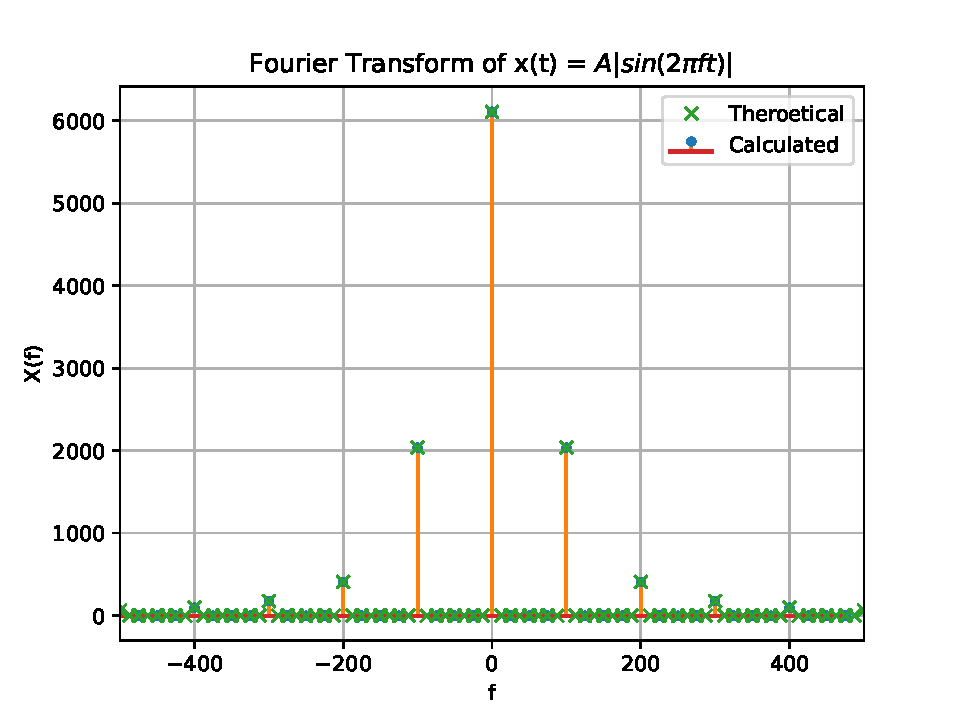
\includegraphics[width=\columnwidth]{./figs/e3.8.pdf}
	\end{center}
	\captionof{figure}{}
	\label{fig:}	
\end{figure}
\vspace{4cm}
 \item Show that 
 \begin{align}
	 \rect{t} \system{F} \sinc{t}
 \end{align}
 Verify using python.\\
\solution 
\begin{align}
	\rect{t}\system{F}\int_{-\infty}^{\infty}\rect{t}e^{-\j2\pi ft}\, dt \\
	=\int_{-\frac{1}{2}}^{\frac{1}{2}}e^{-\j2\pi ft}\, dt \\
	=\frac{e^{\j\pi f} - e^{-\j\pi f}}{\j2\pi f} = \frac{\sin{\pi f}}{\pi f} = \sinc{f}
	\label{eq:fourier-rect}
\end{align}		
\begin{lstlisting}
https://github.com/DarkWake9/EE3900/blob/main/charger/codes/e3.9.py
\end{lstlisting}
\begin{figure}[!ht]
	\begin{center}
		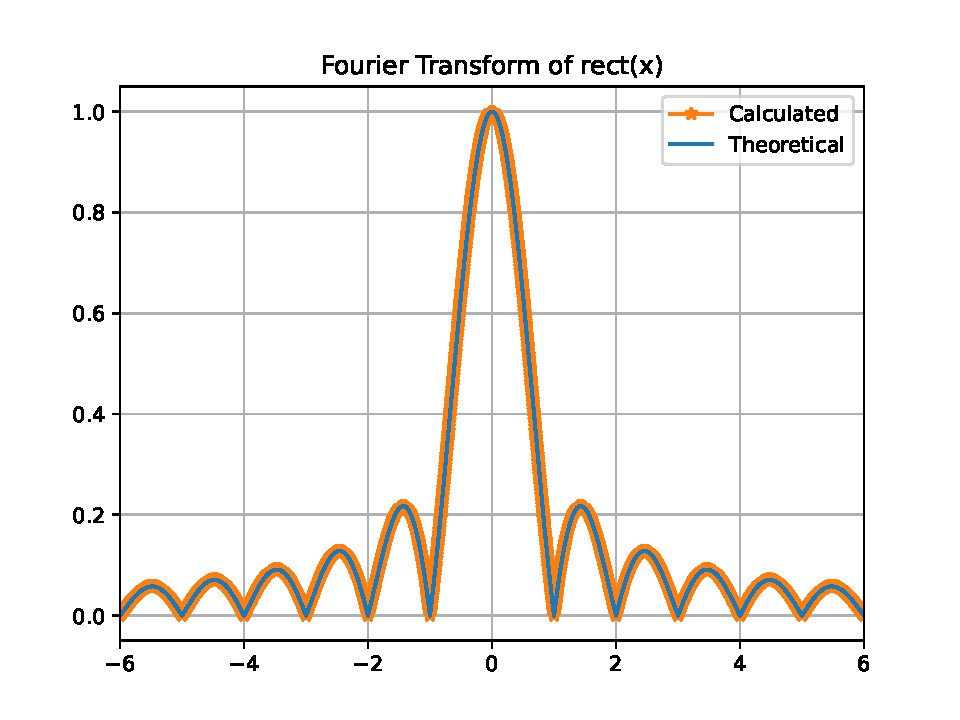
\includegraphics[width=\columnwidth]{./figs/e3.9.pdf}
	\end{center}
	\captionof{figure}{}
	\label{fig:}	
\end{figure}
 \item 
$	 \sinc{t}\system{F} ?$.  Verify using python.\\
\solution From \eqref{eq:duality}
\begin{align}
	\sinc{t}\system{F}\rect{-f}=\rect{f}
	\label{eq:fourier-sinc}
\end{align}
\begin{lstlisting}
https://github.com/DarkWake9/EE3900/blob/main/charger/codes/e3.10.py
\end{lstlisting}
\begin{figure}[!ht]
	\begin{center}
		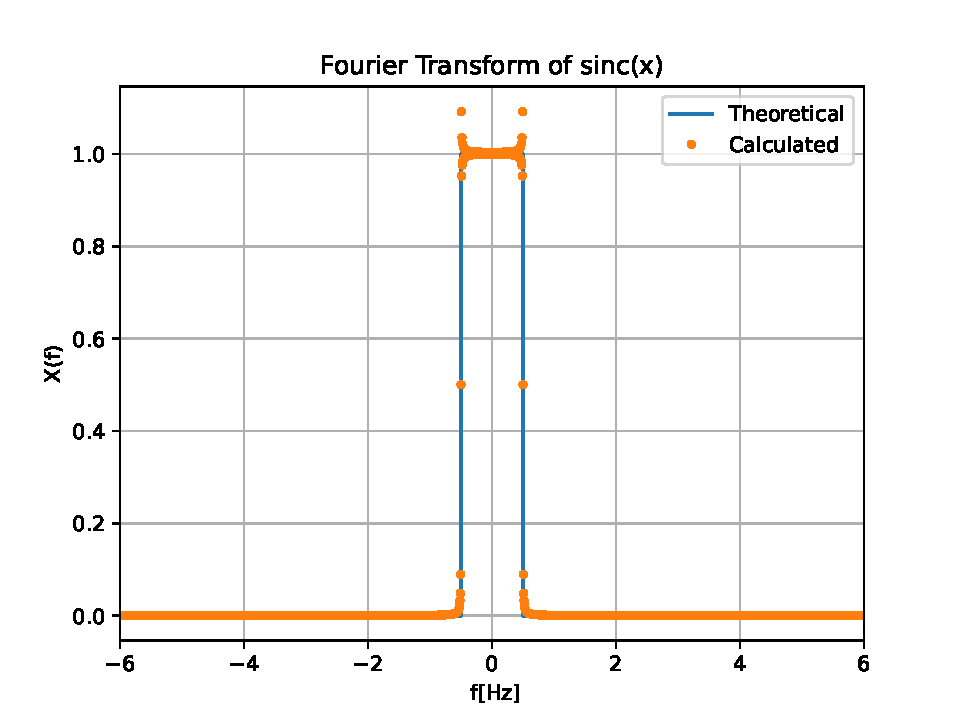
\includegraphics[width=\columnwidth]{./figs/e3.10.pdf}
	\end{center}
	\captionof{figure}{}
	\label{fig:}	
\end{figure}
\end{enumerate}
\section{Filter}
\begin{enumerate}[label=\thesection.\arabic*
,ref=\thesection.\theenumi]
\item Find $H(f)$ which transforms $x(t)$ to DC 5V.\\
\solution\\
H(f) is a \textit{Low-pass} filter which allows only the zero$^{th}$ harmonic and filters the rest.\\

If $f_0$ is the cut-off frequency then an ideal Low-pass filter is described by:
\begin{equation}
	H(f) = \rect{\frac{f}{2f_0}} = \begin{cases}
		1 \quad $if $ \abs{f} < f_0\\
		0 \quad $otherwise$
	\end{cases}
\end{equation}
Multiplying by a scaling factor to get DC 5V,
\begin{equation}
	H(f) = \frac{\pi V_0}{2A_0}\rect{\frac{f}{2f_0}}
		\label{eq:Hf}
\end{equation}
where $V_0 = 5$ V.
\item Find $h(t)$.\\
\solution\\
\begin{align}
	h(t) = \int_{-\infty}^{\infty} H(f)e^{\j2\pi f t}df\\
	= \frac{\pi V_0}{2A_0} \int_{-\infty}^{\infty}\rect{\frac{f}{2f_0}} e^{\j2\pi f t}df\\
	= \frac{\pi V_0}{2A_0} \int_{-f_0}^{f_0} e^{\j2\pi f t}df\\
	= \frac{\pi V_0}{2A_0} \dfrac{e^{\j2\pi f_0 t} - e^{-\j2\pi f_0 t}}{\j2\pi t}\\
	= \frac{\pi V_0}{A_0} \dfrac{\j\sin(2\pi f_0 t)}{\j2\pi t}\\
	= \frac{\pi V_0}{A_0} f_0\sinc{2f_0 t}
\end{align}
\item Verify your result using  through convolution.
\solution
\begin{lstlisting}
https://github.com/DarkWake9/EE3900/blob/main/charger/codes/e4.3.py
\end{lstlisting}
\begin{figure}[!ht]
	\begin{center}
		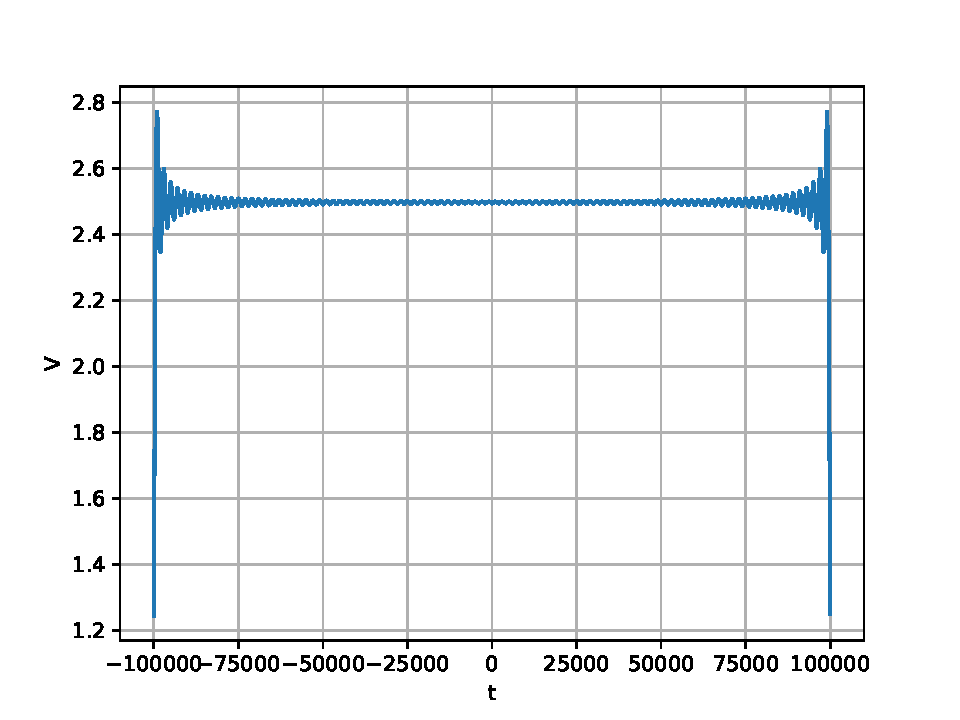
\includegraphics[width=\columnwidth]{./figs/e4.3.pdf}
	\end{center}
	\captionof{figure}{}
	\label{fig:}	
\end{figure}
\end{enumerate}
\section{Filter Design}
\begin{enumerate}[label=\thesection.\arabic*
,ref=\thesection.\theenumi]
\item Design a Butterworth filter for $H(f)$.\\
\solution\\
For an $n^{th}$ order Butterworth filter:\\
The Gain response $G(f)$ is given by\\
\begin{align}
G^2(f) = |H_n(f)|^2 = \frac{1}{1 + \brak{\frac{f}{f_0}}^{2n}}
\end{align}
Where $f_0$ is the cutoff frequency.\\
Gain at a frequency in dB is given as
\begin{align}
	A = -10\log_{10}(G^2(f)) = -20\log_{10}\abs{H_n(f)}
	\label{eq:loss}
\end{align}

Assumptions for the lowpass analog Butterworth filter:
\begin{enumerate}
	\item Passband edge, $f_p = 50$ Hz
	\item Stopband edge, $f_s = 100$ Hz
	\item Passband attenuation, $A_p = -1$ dB
	\item Stopband attenuation, $A_s = -20$ dB
\end{enumerate}
We are required to find a desriable order $n$ and cutoff
frequency $f_0$ for the filter. From \eqref{eq:loss},
\begin{align}
	A_p &= -10\log_{10}\sbrak{1 + \brak{\frac{f_p}{f_0}}^{2n}} \\
	A_s &= -10\log_{10}\sbrak{1 + \brak{\frac{f_s}{f_0}}^{2n}}
\end{align}
Thus,
\begin{align}
	\brak{\frac{f_p}{f_0}}^{2n} = 10^{-\frac{A_p}{10}} - 1 \label{eq:fc1} \\
	\brak{\frac{f_s}{f_0}}^{2n} = 10^{-\frac{A_s}{10}} - 1 \label{eq:fc2}
\end{align}
Therefore, on dividing the above equations and solving for $n$,
\begin{align}
	n = \frac{\log\brak{10^{-\frac{A_s}{10}} - 1} - 
		\log\brak{10^{-\frac{A_p}{10}} - 1}}{2\brak{\log{f_s} - \log{f_p}}}
\end{align}
In this case, making appropriate susbstitutions gives $n = 4.29$.
Hence, we take $n = 5$. Solving for $f_0$ in \eqref{eq:fc1} and
\eqref{eq:fc2},
\begin{align}
	f_{c1} = f_p\sbrak{10^{-\frac{A_p}{10}} - 1}^{-\frac{1}{2n}} = {57.23}{Hz} \\
	f_{c2} = f_s\sbrak{10^{-\frac{A_s}{10}} - 1}^{-\frac{1}{2n}} = {63.16}{Hz}
\end{align}
Hence, we take $f_0 = \sqrt{f_{c1}f_{c2}} = {60}{Hz}$ approximately.
\item Design a Chebyshev filter for $H(f)$.
\solution The Chebyshev filter has an amplitude response
given by
\begin{align}
	\abs{H\brak{f}}^2 = \frac{1}{\brak{1 + \epsilon^2T_n^2\brak{\frac{f}{f_0}}}}
\end{align}
where 
\begin{enumerate}
	\item $n$ is the order of the filter
	\item $\epsilon$ is the ripple
	\item $f_0$ is the cutoff frequency 
	\item $T_n = \cosh^{-1}\brak{n\cosh{x}}$ denotes 
	the n\textsuperscript{th} order Chebyshev polynomial,
	given by
	\begin{align}
		T_n(x) =
		\begin{cases}
			\cos\brak{n\cos^{-1}x} & \abs{x} \le 1 \\
			\cosh\brak{n\cosh^{-1}x} & \textrm{otherwise}
		\end{cases}
		\label{eq:chebypol}
	\end{align}
\end{enumerate}
We are given the following specifications:
\begin{enumerate}
	\item Passband edge (which is equal to 
	cutoff frequency), $f_p = f_0$
	\item Stopband edge, $f_s$
	\item Attenuation at stopband edge, $A_s$
	\item Peak-to-peak ripple $\delta$ in the passband.
	It is given in dB and is related to $\epsilon$ as
	\begin{align}
		\delta = 10\log_{10}\brak{1 + \epsilon^2}
		\label{eq:delta-eps}
	\end{align}
\end{enumerate}
and we must find a suitable $n$ and $\epsilon$.\\
From \eqref{eq:delta-eps},
\begin{align}
	\epsilon = \sqrt{10^{\frac{\delta}{10}} - 1}
	\label{eq:epsilon-del}
\end{align}
At $f_s > f_p = f_0$, using \eqref{eq:chebypol}, $A_s$ is given by
\begin{align}
	A_s = -10\log_{10}\sbrak{1 + \epsilon^2c_n^2\brak{\frac{f_s}{f_p}}} \\
	\implies c_n\brak{\frac{f_s}{f_p}} = \frac{\sqrt{10^{-\frac{A_s}{10}} - 1}}{\epsilon} \\
	\implies n = \frac{\cosh^{-1}\brak{\frac{\sqrt{10^{-\frac{A_s}{10}} - 1}}{\epsilon}}}
	{\cosh^{-1}\brak{\frac{f_s}{f_p}}}
\end{align}
We consider the following specifications:
\begin{enumerate}
	\item Passband edge/cutoff frequency, $f_p = f_0 = {60}{Hz}$.
	\item Stopband edge, $f_s = {100}{Hz}$.
	\item Passband ripple, $\delta = {0.5}{dB}$
	\item Stopband attenuation, $A_s = {-20}{dB}$
\end{enumerate}
$\epsilon = 0.35$ and $n = 3.68$. Hence, we take $n = 4$
as the order of the Chebyshev filter.
\item Design a circuit for your Butterworth filter.
\solution Looking at the table of normalized element values
$L_k$, $C_k$, of the Butterworth filter for order 5, and noting
that de-normalized values $L_k'$ and $C_k'$ are given by
\begin{align}
	C_k' = \frac{C_k}{\omega_c} \qquad L_k' = \frac{L_k}{\omega_c}
\end{align}
De-normalizing these values, taking $f_0 = 60$ Hz,
\begin{align}
	C_1' = C_5' = {1.64}{mF} \\
	L_2' = L_4' = {4.29}{mH} \\
	C_3' = {5.31}{mF} \\
\end{align}
The L-C network is shown in Fig. \ref{fig:butter-filter}.
\begin{figure}[!ht]
	\centering
	\begin{circuitikz} 
		\draw (0,0) to[short, o-o] (7,0);
		\draw (0,2) to [short, o-] (1,2) to [L, l=4.29 mH] (3.5,2) to [L, l=4.29 mH] (6,2) to[short, -o] (7,2);
		\draw (1,0) to[C, l=1.64 mF] (1,2);
		\draw (3.5,0) to[C, l=5.31 mF] (3.5,2);
		\draw (6,0) to[C, l=1.64 mF] (6,2);
	\end{circuitikz}
	\caption{L-C Butterworth Filter}
	\label{fig:butter-filter}
\end{figure}
\\
Python code to compare the amplitude response
of the simulated circuit with the theoretical expression.
\begin{lstlisting}
https://github.com/DarkWake9/EE3900/blob/main/charger/codes/e5.3.py
\end{lstlisting}
\begin{figure}
	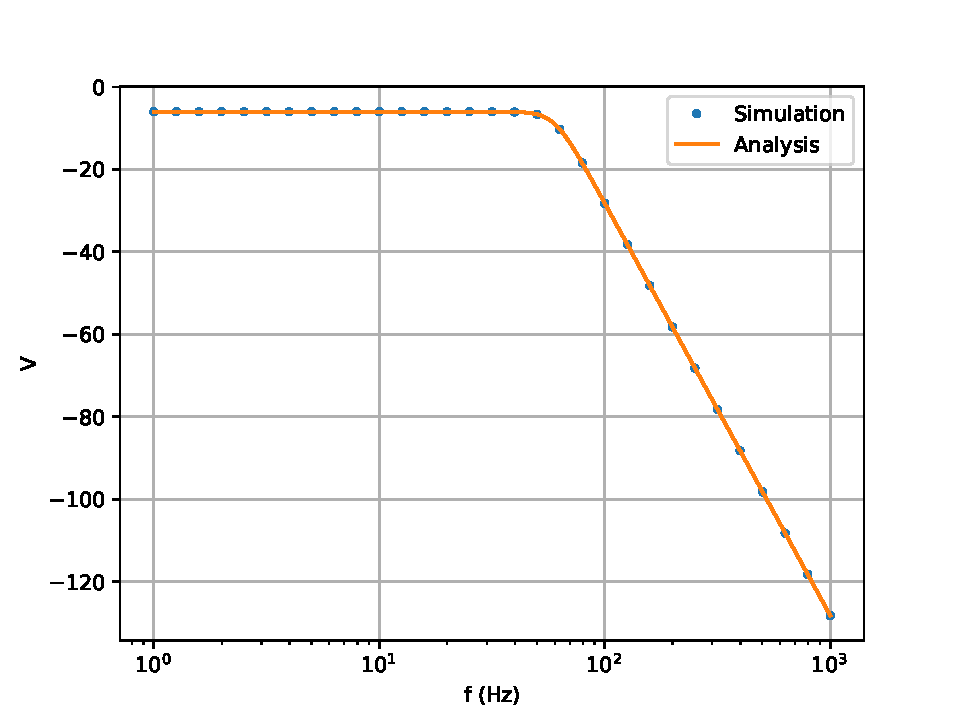
\includegraphics[width=\columnwidth]{figs/e5.3.pdf}
	\caption{Amplitude Response of Butterworth filter.}
	\label{fig:sim-butter}
\end{figure}
\vspace{2cm}
\item Design a circuit for your Chebyshev filter.
\solution Looking at the table of normalized element values
of the Chebyshev filter for order 3 and 0.5 dB ripple,
and de-nomrmalizing those values, taking $f_0 = {60}{Hz}$,
\begin{align}
	C_1' = {4.43}{mF} \\
	L_2' = {3.16}{mH} \\
	C_3' = {6.28}{mF} \\
	L_4' = {2.23}{mH}
\end{align}
The L-C network is shown in Fig. \ref{fig:cheby-filter}.
\begin{figure}[!ht]
	\centering
	\begin{circuitikz} 
		\draw (0,0) to[short, o-o] (7,0); 
		\draw (1,0) to[C, l=4.43 mF] (1,2);
		\draw (3.5,0) to[C, l=6.28 mF] (3.5,2);
		\draw (0,2) to [short, o-] (1,2) to [L, l=3.16 mH] (3.5,2) to[L, l=2.23 mH] (6,2) to[short, -o] (7,2);
	\end{circuitikz}
	\caption{L-C Chebyshev Filter}
	\label{fig:cheby-filter}
\end{figure}

Python code to compare the amplitude response
of the simulated circuit with the theoretical expression.
\begin{lstlisting}
https://github.com/DarkWake9/EE3900/blob/main/charger/codes/e5.4.py
\end{lstlisting}
\begin{figure}
	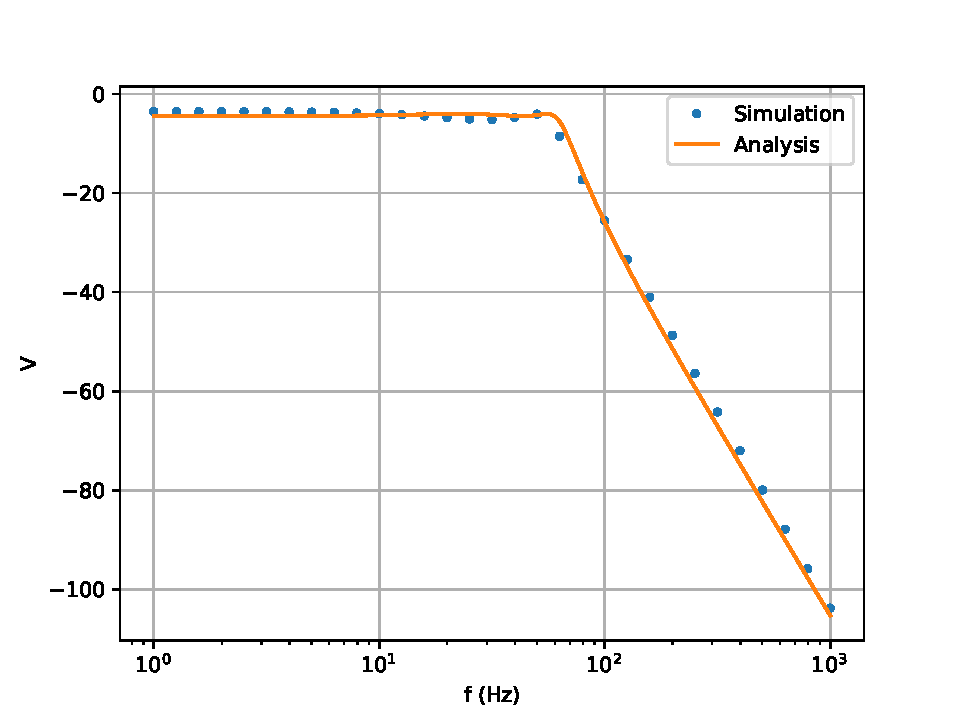
\includegraphics[width=\columnwidth]{figs/e5.4.pdf}
	\caption{Amplitude Response of Chebyshev filter.}
	\label{fig:sim-cheby}
\end{figure}
\end{enumerate}
\end{document}
